%%%%%%%%%%%%%%%%%%%%%%%%%%  phdsymp_sample2e.tex %%%%%%%%%%%%%%%%%%%%%%%%%%%%%%
%% changes for phdsymp.cls marked with !PN
%% except all occ. of phdsymp.sty changed phdsymp.cls
%%%%%%%%%%                                                       %%%%%%%%%%%%%
%%%%%%%%%%    More information: see the header of phdsymp.cls   %%%%%%%%%%%%%
%%%%%%%%%%                                                       %%%%%%%%%%%%%
%%%%%%%%%%%%%%%%%%%%%%%%%%%%%%%%%%%%%%%%%%%%%%%%%%%%%%%%%%%%%%%%%%%%%%%%%%%%%%%
%\documentclass[10pt]{phdsymp} %!PN
\documentclass[twocolumn]{phdsymp} %!PN
%\documentclass[12pt,draft]{phdsymp} %!PN
%\documentstyle[twocolumn]{phdsymp}
%\documentstyle[12pt,twoside,draft]{phdsymp}
%\documentstyle[9pt,twocolumn,technote,twoside]{phdsymp}
 
\usepackage[english]{babel}       % Voor nederlandstalige hyphenatie (woordsplitsing)

\usepackage{graphicx}                   % Om figuren te kunnen verwerken
\usepackage{graphics}			% Om figuren te verwerken.
\graphicspath{{figuren/}}               % De plaats waar latex zijn figuren gaat halen.
\usepackage{booktabs}
\usepackage{times}
\usepackage[margin=1cm]{caption}
\usepackage{float}
\usepackage{caption}
\usepackage{subcaption}
\usepackage{tabularx}
\hyphenation{si-mu-la-ted re-a-lis-tic packets really in-clu-ding}

\def\BibTeX{{\rm B\kern-.05em{\sc i\kern-.025em b}\kern-.08em
    T\kern-.1667em\lower.7ex\hbox{E}\kern-.125emX}}

\newtheorem{theorem}{Theorem}

\usepackage[language=english, sorting=none]{biblatex}
\setlength{\tabcolsep}{12pt}
\renewcommand*{\bibfont}{\small}
\addbibresource{references.bib}
\usepackage{enumitem}


\begin{document}

\title{Design and development of a health recommendersystem focussing on rope skipping} %!PN

\author{Elise Thienpont}


\supervisor{Toon De Pessemier, Luc Martens}

\maketitle

\begin{abstract}
Physical activity is vital in our sedentary society. However, this is difficult to achieve without any form of personal coaching. Nowadays everyone has some kind of mobile device in their possession. This is a source of possibilities in terms of physical activity coaching. A smartwatch adds an extra dimension by directly monitoring physical activity by making use of heart rate sensors. This data makes it possible to also produce personal recommendations.
One of the most frequently used arguments in favor of too little movement, is the lack of time. Rope skipping is the ideal solution for this problem. This sport ensures optimal endurance training so that users can train efficiently. The sport can also be carried out anywhere provided there is enough space. As far as movement recognition of specific rope skipping movements is concerned, very little research has been carried out. However, by recognizing the movements and detecting possible shortcomings, additional encouragement can be provided.
This paper describes an Android application developed to teach the user a healthy movement pattern. This accomplished with the addition of the rope skipping element.
The developed rope skipping recognition model is able to predict movements with an accuracy of 96\%.
\end{abstract}

\begin{keywords} rope skipping, health application, wear OS, android, recommender system, machine learning, neural network
\end{keywords}

\section{Introduction}
\PARstart{S}{port} and exercise are gaining popularity in our society. More people are therefore using mobile applications to improve their performance in various areas related to sport and general health. \\
\noindent
However, current health applications often only provide static recommendations. They do not take the user's personal progress, his or her condition and physical abilities into account. Users must therefore specify their desired objectives themselves. Based on these parameters, the application will then give corresponding recommendations. \\
\noindent
Rope skipping is a sport that keeps the user in good shape and requires little space or time. The sport is therefore ideal to encourage people to exercise more frequently. An in-depth research of this activity concerning movement recognition has however never been conducted. \\
\noindent
If and when the user exceeds his or her physical limits, voluntarily or due to unhealthy circumstances, is usually not reported. This can cause long-term damage, which is certainly not beneficial to the health. A classification of the user context in terms of health status is consequently necessary. \\
\noindent
The main goal of this thesis is to develop a mobile application that teaches users a healthy lifestyle by means of personal recommendations. These recommendations will clarify what the user must do to maintain optimal health. The content of these recommendations is based on the physical activities of the user and what his or her current condition allows (personalized). This research will focus on rope skipping as this achieves the objective of the thesis. \\

\noindent
The main contributions of this paper are as follows:\\
\begin{itemize}[leftmargin=.1in]
\raggedright
\setlength\itemsep{0.7em}
    \item Accurate rope skipping movement classification
    \item Producing personalized recommendations
    \item Integrating these components into an android application
\end{itemize}
\bigskip 


\section{Related work}

\Cite{ref13} conducts research to find the most optimal window size and sampling frequency. However, this is highly dependent on the type of activity. Windows from 0.5 to 17 seconds are possible. 
The ideal combination of window size and sampling frequency was found by applying the model to and comparing the following categories: gender, age and BMI. These subdivisions gave similar results, namely a window size of 10 seconds and a sampling frequency of 50 Hz.\\
In an initial phase of the research conducted during this thesis, the optimal window format found in this study was used. The idea of removing partial windows was also adopted. 

In \cite{ref15} a trade-off is made between the number of sensors and the classifier used. The use of multiple sensors (e.g. sensors on the wrist and chest) results in reduced ease of use. Using multiple sensors also results in obstruction of movements and an impractical element during long-term use. Previous studies have proven that multiple sensors are disadvantageous to identifying human activities. It has also been proven that accelerometer data is sufficient to complete the classification. \\
Consequently, during this research, only a smartwatch sensor will be used to ensure optimal ease of use. The research also focuses on accelerometer data. In an initial phase of the study, an overlap of 50\% was used. The study discussed has also shown that dimensionality reduction promotes accuracy. Consequently, this was applied during the thesis when necessary. \\

\cite{ref17} is an example of an online activity recognition system.
Data processing can be done on the mobile device itself, but there are limitations due to limited hardware (less data that can be buffered), the robustness of classification algorithms and the number of events that can be classified (energy consumption). However, this thesis focuses on a limited number of specific rope skipping movements. Energy consumption will therefore not be an obstacle. Contemporary smartphones are also able to perform more complex calculations.

A number of studies on activity recognition train a model consisting of, among others, the simple forward jump. However, research into specific rope skipping movements is lacking.

In  \cite{ref53} research is done into the recognition of daily activities. This study comes superficially into contact with rope skipping.

Different people can perform the same activity, but the level of effort varies greatly. Subsequent studies look for a metric to represent this level of activity.

In \cite{ref18}, oxygen utilization (VO2) was used as a metric for physical exhaustion. Children performed activities with an indirect calorimeter. This is a gas analysis system that measures the volume of exhaled air as well as the O2 and CO2 concentration. An accelerometer (AG) and a heart rate monitor are also used sensors. Differences in VO2 and AG vector magnitude were measured.
With this data, the number of METs is calculated by dividing the average VO2 consumption by the predicted RMR (Resting Metabolic Rate).
Due to the lack of means to measure oxygen consumption, this method cannot be applied in the context of this thesis.

The application developed in \cite{ref21} will give personal suggestions for physical activity. A goal is calculated every week based on whether goals have been achieved in previous weeks or not and on the basis of SE beliefs. SE beliefs are answers to questions asked to the user about the activity performed. The SE score is the average of the answers given. The goal is expressed in METs based on heart rate. The duration of the average intensity zone (6 * MAXHR/10, 7 * MAXHR/10) and the length of time in the intensive zone (7 * MAXHR/10, 8 * MAXHR/10) are examined. The general guidelines say that 600 METs per week is required to live a healthy life. This heart-based method is very suitable for use during this thesis. Consequently, the method was applied. The idea of obtaining a more personal goal through SE beliefs is not applied. This is because the application developed in this thesis needs to function automatically.

The presence of a target is essential for the operation of a health application. This way, the personal aspect is realized.
Dynamic goal setting can be accomplished through complex machine learning algorithms or simpler heuristics. 

In \cite{ref11}, goals are set on the basis of reinforcement learning. Setting goals is an important factor in causing significant change in behavior. Dynamic goals can be accomplished by simple heuristics such as taking the 60th percentile of the steps taken in the past 10 days. A more complex way makes use of reinforcement learning. The behavioral analytics algorithm uses inverse reinforcement learning to obtain a model from historical data. After this, the model is used to generate realistic goals.
This thesis uses an average value for the calculation of goals. Since the algorithm will be implemented in Android, an additional machine learning model is overkill.

In \cite{ref23}, a widget was created that stores user activity and predicts what actions the user will take. The data that is viewed are text messages, telephone calls and applications used. The recommendation algorithm is fully focused on SQL functionality. For example, when recommending the most likely phone call, the total duration of each call is filtered by day of the week and grouped by contact number. The greatest duration is then given as a prediction.
The recommendation algorithm in this thesis was developed according to the approach in this study.

\section{Rope skipping}

\subsection{Movements}
The investigated movements are the following: jump fast, jump slow, side swing, cross over and jump run. Jump fast, jump slow and jump run are variations of the same movement since regular jumping can be performed fast, slow or while running. These variations are distinct enough to classify them separately.

\subsection{Data collection}
The polar M600 smartwatch is used in combination with an android smartphone for data collection purposes.
Since the polar flow platform however does not allow downloading of raw data \cite{ref28}, an own application was developed on the smartwatch and smartphone. The smartwatch application will receive data points via sensors with a sampling frequency of approximately 52 Hz.

Every time a data point comes in, it is sent to the smartphone via the wear OS message Client. The data points are sent in this way because they can then be saved to a CSV file via an application on the Android smartphone. This process is more efficient on a smartphone compared to a smartwatch. The data file can then be found in the internal storage of the smartphone.

\subsection{Machine learning algorithm research}
There is a wide variety of machine learning algorithms and since it is not a simple task to chose the right one based solely on theoretical knowledge, a researched was conducted. 

\subsubsection{Preprocessing}
\noindent\textbf{Data Quality Assessment}\newline
To filter out data corresponding to turning the smartwatch on and off during a measurement, the first and last data points are deleted in an interval of 3 seconds. These data points do not belong to any class and will just confuse the machine learning model.

Duplicates are noticed when observing the data values, which is an error in the data collection process. However, this is not a problem as duplicates can easily be detected and removed via the pandas framework.

Data collection by sensors in a smartwatch does not require human interaction, so the chance of missing values is small. Rows to which NaN values belong are therefore removed.

Some precautions are taken by converting the x, y and z feature into float objects. This to make sure that the data is consistent. \\

\noindent\textbf{Feature aggregation}\newline
The resulting data set is initially divided into 1 second segments each with 50 percent overlap. One full jump will take just under one second on average. Hence the choice for a segment size of one second. This will be further investigated in section \ref{section:cnn}. \\

\noindent\textbf{Feature extraction}\newline
Just the x, y and z component of an acceleration vector is not enough for most algorithms to make correct predictions. Therefore, based on the data points in a segment, a number of new features are extracted. By calculating SMV, SMA, tilt angle, PSD and a number of statistical features a total of 21 features are extracted. \\

\noindent\textbf{Dimensionality reduction}\newline
Because many algorithms cannot deal with big dimensionality, dimensionality reduction is applied during this research. A value of 6 was chosen for the number of dimensions. \\

\noindent\textbf{Feature encoding}\newline
When identifying activities, individual data points must be compared. In order to accurately compare the data points they must be transformed so that they have an equal distribution. This can be accomplished by normalizing every data point individually.

The ground truth labels in the form of rope skipping movements must also be encoded. This is achieved using the labelEncoder module from Scikit Learn. \\

\noindent\textbf{Data balancing}\newline
In an initial phase of the study, balancing was done by making each class as big as the smallest one. Later data augmentation is used to solve this problem. \\

\noindent\textbf{Data variation}\newline
The same movement can be measured in different ways. For example, the distinction can be made between the wrist on which the smartwatch is worn or between the direction of rotation.
Movements such as forward 180, backward 180 and jump run can't be practiced with a reverse direction. Consequently, the variations do not apply to these movements.
Including these variations in the training data will result in a better model. Since these essentially represent the same movement.  \\

\noindent\textbf{Validation dataset}\newline
By means of a classic train/test split a train and test dataset was created. At this point in the research no validation dataset was used. During CNN optimisation (section \ref{section:cnn}) validation data consisted of movements carried out at different times to ensure diversity. \\

\noindent\textbf{Classifier evaluation}\newline
The algorithms used are the following: SVC, lineairSVC, Random forest, Adaboost, Naive bayes, K-nearest neighbors, SGD, MLP and finally CNN. This research showed that CNN was the best fit for the dataset used in this study as shown in Table \ref{tab:CNN}.  

\begin{table}[!htpd]
  \centering
  \caption{Performance}
  \label{tab:CNN}
\begin{tabular}{lccc}
 \hline \\
\textbf{}             & \textbf{Precision} & \textbf{Recall} & \textbf{F1} &  \\
\hline \\
\textbf{SVC}                 & 0.66               & 0.67            & 0.65        &  \\
\textbf{LineairSVC}         & 0.66               & 0.62            & 0.57        &  \\
\textbf{Random Forest}       & 0.74               & 0.75            & 0.74        &  \\
\textbf{Adaboost}           & 0.76               & 0.76            & 0.76        &  \\
\textbf{Naive Bayes}         & 0.60               & 0.61               & 0.58        &  \\
\textbf{K-nearest neighbors}   & 0.58                  & 0.61            & 0.59        & \\
\textbf{SGD}                    & 0.58                  & 0.60            & 0.59        & \\
\textbf{MLP}                    & 0.63                  & 0.65            & 0.64       & \\
\textbf{CNN}                     & 0.90                  & 0.90            & 0.90        & \\
\hline \\
\end{tabular}
\end{table}

\subsection{CNN optimisation} \label{section:cnn}
CNN proved to deliver the best results by far with the classic train test split. 
At this point it was decided not to further investigate the forward and backward 180 movements in the context of this thesis.
The reasoning behind this choice is as follows: The final health application will recommend sessions of one particular activity. However, the forward and backward 180 are movements that are difficult to perform periodically. There was also considerable confusion between backward 180, forward 180 and jump slow. This is due to the similarity of these movements.
To compensate for the loss of the forward 180s, a replacement movement was sought. The jump run is a good candidate. \\

\noindent\textbf{Window}\newline
One of the hyperparameters that can be tinkered with is the window. In previous experiments, a one second window was used. This because a single jump always has a duration of about one second. Table \ref{tab:window} shows the accuracy of the model with respect to window size. This accuracy is an average score. Since as mentioned one jump has an average duration of one second, it is logical that a window of half a second gives slightly worse results. A window larger than 1 will cause problems when different movements follow each other in quick succession. For this reason, segments of 1 second were chosen. \\

\begin{table}[!htpd]
  \centering 
  \caption{Window evaluation}
  \label{tab:window}
\begin{tabular}{lccccc}
 \hline \\
\textbf{}         & \textbf{0.5 s} & \textbf{1 s} & \textbf{1.5 s} & \textbf{2 s} & \textbf{3 s} \\\\
 \hline \\
\textbf{Accuracy} & 0.83           & 0.90         & 0.89           & 0.92         & 0.93  \\\\
 \hline \\
\end{tabular}
\end{table}

\noindent\textbf{Overlap}\newline
Furthermore, experiments were carried out with overlapping or non-overlapping segments during training. Previous experiments each worked with a 50\% overlap of both training and validation dataset. A certain overlap will ensure that on the one hand more training data is available and on the other hand all the characteristics of the signal are modeled. However, too much overlap will cause overfitting. The results can be seen in table \ref{tab:overlap}. It was decided to continue working with an overlap of 30\%. \\

\begin{table}[!htpd]
  \centering
  \caption{Overlap evaluation}
  \label{tab:overlap}
\begin{tabular}{lcccc}
 \hline \\
\textbf{}         & \textbf{0\%} & \textbf{30\%} & \textbf{50\%} & \textbf{70\%} \\\\
 \hline \\
\textbf{Accuracy} & 0.88         & 0.93          & 0.90          & 0.93   \\\\
 \hline \\
\end{tabular}
\end{table}

\noindent\textbf{Dividing}\newline
A subsequent experiment consisted of splitting into multiple models based on the variations in the training data. Four models were trained, each specialized in one specific type of data. Accuracy increased in most models as a result. However, there was still some confusion between backward and forward 180.
With the implementation of the android application in mind, it was decided to train only one model. In the case of four models trained on different data, the user would have to specify which variation to perform (left wrist-backward, right wrist-forward ...). As a result, this approach is certainly not user-friendly. \\

\noindent\textbf{Merging classes}\newline
In this section it is investigated if classification is possible when jump fast and jump slow are merged into one class.
The reasoning behind initially splitting jump slow and jump fast is as follows: these movements show enough distinction among themselves to be classified separately and the calculation of the number of turns is also based on this distinction. Namely, the parameters used are different. Table \ref{tab:merging} shows that the merging makes classification for the model somewhat more difficult. \\

\begin{table}[!htpd]
  \centering
  \caption{Merging jumps}
  \label{tab:merging}
\begin{tabular}{lccc}
 \hline \\
\textbf{}             & \textbf{Precision} & \textbf{Recall} & \textbf{F1} &  \\
 \hline \\
\textbf{Jump run}  & 0.64               & 0.79            & 0.71        &  \\
\textbf{Jump}       & 0.97               & 0.87           & 0.92        &  \\
\textbf{Cross over}   & 0.27               & 1               & 0.43        &  \\
\textbf{Side swing}   & 0.79                  & 0.99           & 0.88        & \\
 \hline \\
\end{tabular}
\end{table}

\noindent\textbf{Ensemble learning}\newline
Ensemble learning is a way to eliminate errors from individual models. Every new run of the same model will never be equal to a previous one. This is caused by random weight initializations. Four models are trained in the same way with the same input data. These models will work together to find a solution in the following manner. When a model makes a prediction, a probability is assigned to each of the classes. These probabilities, coming from the four models, are added together so that each model contributes to the final result. The class with the highest score is assigned to the segment. The result of this can be seen in Figure \ref{fig:model} and Table \ref{tab:model} \\

\begin{table}[!htpd]
  \centering
  \caption{Ensembled model performance}
  \label{tab:model}
\begin{tabular}{lccc}
 \hline \\
\textbf{}             & \textbf{Precision}  & \textbf{Recall}   & \textbf{F1} &  \\
 \hline \\
\textbf{Jump run}     & 1                   & 0.82              & 0.90       &  \\
\textbf{Jump slow}    & 0.91                & 1                 & 0.95       &  \\
\textbf{Jump fast}    & 1                   & 1                 & 1       &  \\
\textbf{Cross over}   & 1                   & 1                 & 1        &  \\
\textbf{Side swing}   & 0.92                & 1                 & 0.96       & \\
 \hline \\
\end{tabular}
\end{table}

\begin{figure}[!htpd]
\centering
\caption{Ensembled model}\label{fig:model}
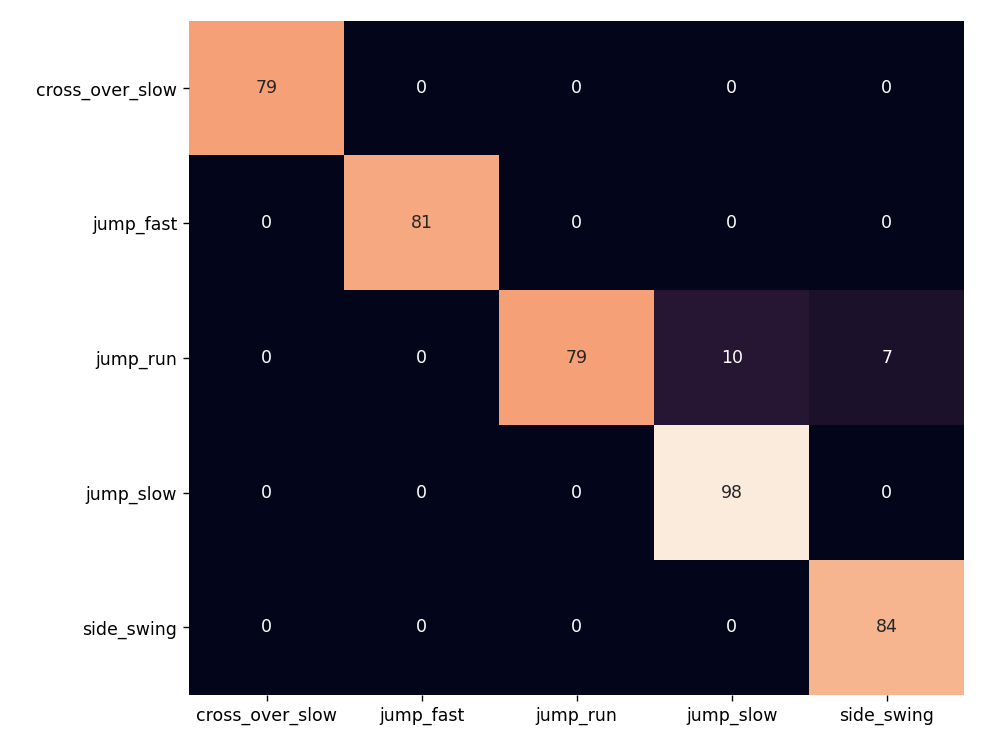
\includegraphics[width=.4\textwidth]{images/confusion_matrix_final.PNG}
\end{figure}

\section{Health application}
In this section the development of the health application is further explained. First the calculation of the number of turns and mistakes is explained. Subsequently, a overview of the resulting health application is given.

\subsection{Turns}
The number of turns in a rope skipping session can be obtained by looking at the period of the signal. This period will be the same over x, y and z axis.
To calculate the number of periods and thus the number of turns, a Savitzky Golay filter is used. This will ensure that there is only one local maximum per period. By performing a peak detection on this smooth signal, a fairly good approximation can be made of the effective number of turns. The average is calculated between the three axes.

\subsection{Mistakes}
When an error occurs during a session in the form of an altered rotation, this is clearly noticeable in the course of the signal. There will be no or barely any acceleration visible for a few seconds. By first taking the derivative of the signal it is possible to filter data points in an interval close to zero. If a series contains enough values, this is labeled as an error. Through an empirical study, this parameter was set at 52 data points. The error detection interval was set at a lower limit of -0.0000001 and an upper limit of 0.0000001.

\subsection{Smartwatch application}
The smartwatch application is responsible for starting sessions and collecting data during these sessions. The accelerometer and heart rate data points are sent via the MessageClient API to the android application running on a smartphone. Since measurements are done at a frequency of 52Hz, sending data points in real time can have an impact on the battery life and/or performance of the application. For these reasons, it is decided to send the data in batches of 104 data points.
During a session, the heart rate is also monitored, if it becomes dangerously high, the smartwatch will signal this via a vibration. Figure \ref{fig:smartwatch} shows the smartwatch interface.

\begin{figure}[!htpd]
\centering
  \caption{Smartwatch session} \label{fig:smartwatch}
  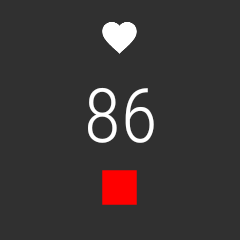
\includegraphics[width=.2\textwidth]{images/smartwatch-session.png}
\end{figure}

\subsection{Smartphone application}
The smartphone application is responsible for receiving data points and processing them. The machine learning model is available locally and is therefore used to recognize movements in the received accelerometer data. The number of turns and possible errors are also calculated. The number of MET minutes per movement will be calculated using heart rate data points within a time interval determined by the duration of a session. These are later used to generate recommendations.
These recommendations will be calculated every week on the basis of historical data. These can be seen on the application so the user can choose when to perform a recommended activity. A recommendation can be converted into an effective session which is initiated by a message sent to the smartwatch application. The accompanying recommendation is put on pending so that it can be checked whether the user has actually completed it. It is checked whether the duration of the activity corresponds to the recommended duration and whether the effort level is more or less the same.
A finished recommendation is set to done and displayed in gray within the application. Figure \ref{fig:pending} and \ref{fig:timeline} show a visualisation of the pending recommendations and the timeline of activities.

\begin{figure}[!htpd]
\centering
\begin{floatrow}
  \ffigbox{\caption{Pending recommendations}\label{fig:pending}}{%
    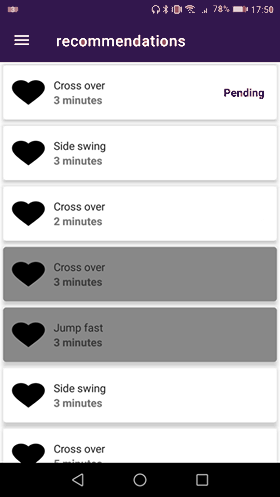
\includegraphics[width=.17\textwidth]{images/pending_recommendations.png} 
  }
  \ffigbox{\caption{Timeline activities}\label{fig:timeline}}{%
    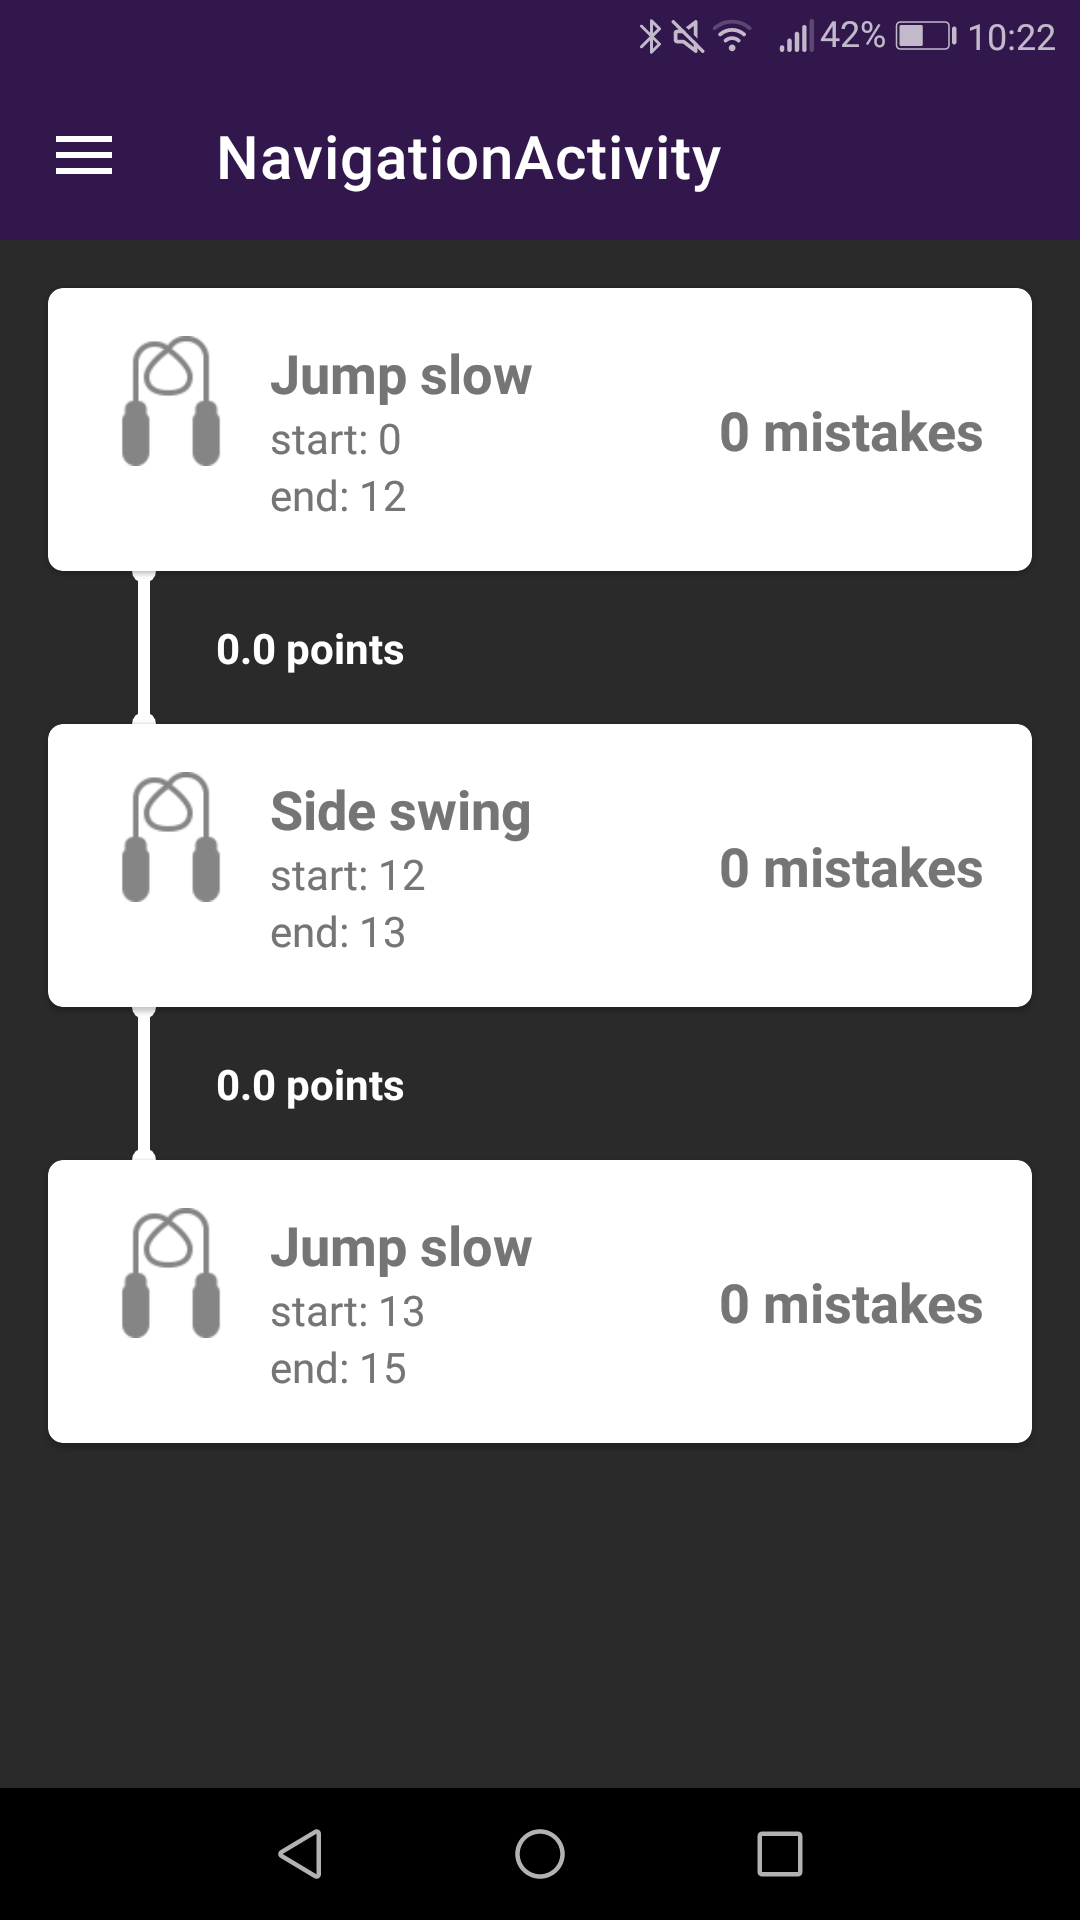
\includegraphics[width=.17\textwidth]{images/timeline.png} 
  }
\end{floatrow}
\end{figure}

\subsection{Recommendations}
The system developed during this thesis emphasizes the personal aspect. Therefore, a content-based method is aimed at the user is chosen. There are only a limited number of movements. So there is a good chance that one user will perform them all. However, there will be some inconvenience from a cold start. No information is yet known about a new user. Therefore, a number of random recommendations are generated so that the system can learn in the long-term.

A new set of recommendations is calculated every week. The developed algorithm takes into account the number of sessions in which a certain activity has been performed. The number of errors made during a movement is also taken into account. We work with a system that assigns weights to each activity based on the above criteria. The duration of a recommendation is equated with the average duration of the chosen activity based on historical data. The total number of MET minutes of all calculated recommendations added together must be equal to or greater than the goal associated with that week. This total number of METs is obtained by using the average number of METs per second for each corresponding activity and adding them up each time.
If sessions are not yet available, the capabilities and preferences of the user cannot yet be taken into account. An equal weight is assigned to each activity. For the same reason, the duration of an activity is chosen at random within the five to ten minute interval. This turned out to be an acceptable duration for novice rope skippers after some research. It is important not to let the initial duration of the random recommendations last too long. An amateur rope skipper may or may not be discouraged by overestimating his/her abilities. The goal is set at the healthy value of 600 MET minutes per week when no data is yet available.

\subsection{Score}
A MET score is linked to the activity based on the time spent in each heart rate zone. This gives an accurate picture of how difficult the activity was for the user. Following formula is used to calculate the score. 
\[METminutes = 4*timeMPA + 8*timeVPA\] 
TimeMPA and timeMVPA respectively represents the time spent in the moderate activity zone and the time spent in the vigorous activity zone \cite{ref21}.


\subsection{Goal calculation}
The target for the following week is calculated by looking at historical data up to ten weeks in the past. This data shows how many METs the user has consumed per week. The average is taken from this. This so the goal does not rise or fall too sharply and thus remains within the limits of possibilities. When not enough data is available, the historical data is supplemented with a value of 600 METs. According to the literature, this is the recommended MET consumption per week \cite{ref21}.

\section{Evaluation}
In order to complete the evaluation efficiently, some adjustments have been made. The recommendations, which are usually calculated weekly, will be calculated daily. The target will therefore also be adjusted daily. The default value for this is set to the rounded value of 85 MET minutes. Two test subjects will use the designed application for several days. This in such a way that the final working conditions can be simulated. Every day a number of sessions will take place. 

\subsection{Turns and mistakes}
Evaluation of the number of turns and recorded errors was done according to an empirical study. The parameters were adjusted each time so that the outcome was closer to reality. The time spent during an error was also examined. It was concluded that the time between stopping with jumping due to an error and restarting was about one second. Table \ref{tab:turns} and  \ref{tab:mistake} gives an overview of the final results.

\begin{table}[!htpd]
    \centering
    \begin{tabular}{lc}
    \hline \\
    \multicolumn{1}{c}{\textbf{}}          & \textbf{Margin of error} &\\
     \hline \\
    \multicolumn{1}{c}{\textbf{Jump run}}  & 2                    &\\
    \multicolumn{1}{c}{\textbf{Jump slow}} & 2                    &\\
    \textbf{Jump fast}                     & 3                    &\\
    \textbf{Side swing}                    & 1                   & \\
    \textbf{Cross over}                    & 1  & \\
 \hline \\
    \end{tabular}
    \caption{Turn detection}
    \label{tab:turns}
\end{table}

\begin{table}[!htpd]
    \centering
  \begin{tabular}{lc}
 \hline \\
    \textbf{}               & \textbf{Amount} &\\
     \hline \\
    \textbf{True positive}  & 11                &\\
    \textbf{False positive} & 3                 & \\
    \textbf{False negative}  & 2               &\\
 \hline \\
    \end{tabular}
    \caption{mistake detection}
    \label{tab:mistake}
\end{table}

\subsection{Recommendations}
A first subject with an average fitness evaluated the application for three days. The focus was on the jumps side swing and jump fast. This was reflected in the recommendations given after the first day. Since the sessions were short in duration and required minimal effort, the target set was not met. This was reflected in the proposed target for the next day, which was 51 MET minutes. This pattern was maintained for two additional days. The recommendations adapted to the preference of the user and the desired duration.
A second subject with worse condition also evaluated the application for three days. The user was only able to perform a side swing. This preference was clearly reflected in the recommendations. After the first day, the goal dropped by just 9 MET minutes. This phenomenon continued over the next few days, ending with a goal of 60 MET minutes. This small decrease can be explained by the older age of this subject. Because at this age a high heart rate zone is reached faster.

\section{Conclusions}
\noindent
This thesis investigated the possibilities in regards to recognition of rope skipping movements. Due to limited access to different sensors, only wrist movements could be examined, which reduced the number of movements that could be investigated.
Notwithstanding, it was proven that rope skipping movements differ from each other purely with data from wrist movements. In a first phase, it was investigated which machine learning algorithm is most suitable for this classification problem. The convolutional neural network, CNN for short, gave the best results. Then, applied to CNN, the most optimal window size was examined. This started from the hypothesis that a jump takes an average of one second, which was confirmed during the investigation. Windows of one second and more turned out to provide good accuracy. Subsequently, it was investigated which amount of overlap ensures the highest performance. This showed that some overlap is beneficial. Overlaps of 30, 50 and 70 percent resulted in similar accuracy. 30\% was chosen because of the risk of overfitting at higher percentages.
It was also investigated to what extent variations within a class result in a decrease in accuracy. After splitting, a slight increase in accuracy was noted in the individual models.
As a last experiment, the effect of ensemble learning on the performance was examined. It was found that multiple collaborating models provide higher accuracy.

Subsequently, this model was used in the context of a health application. It was demonstrated that recommendations can be produced based on effort points and the user's personal preference. More encouragement was also provided through the display of errors and number of turns.

\section{Limitations and Future Work}
Despite the good results, there are still a few options with regard to future work.
Due to the corona measures, it turned out to be impossible to obtain sufficient test subjects. Future studies can further generalize the developed model in this way. The health application can also take into account the stress level and sleep pattern of the user. In this way, the recommendations can be made even more personal. User context regarding the weekly pattern can also be taken more into account.

\nocite{*}
\bibliographystyle{phdsymp}
%%%%%\bibliography{bib-file}  % commented if *.bbl file included, as
%%%%%see below


%%%%%%%%%%%%%%%%% BIBLIOGRAPHY IN THE LaTeX file !!!!! %%%%%%%%%%%%%%%%%%%%%%%%
%% This is nothing else than the phdsymp_sample2e.bbl file that you would%%
%% obtain with BibTeX: you do not need to send around the *.bbl file        
%%
%%---------------------------------------------------------------------------%%
%

\printbibliography


\end{document}

%%%%%%%%%%%%%%%%%%%%%  End of phdsymp_sample2e.tex  %%%%%%%%%%%%%%%%%%%%%%%%%%%


